\documentclass[a4paper,11pt]{article}

\usepackage[T1]{fontenc}
\usepackage[utf8]{inputenc}

% IWCS
% included below \usepackage{graphicx}  %%% for including graphics
% included below \usepackage{url}       %%% for including URLs
\usepackage{times}
% included below: \usepackage{natbib}
\usepackage[margin=25mm]{geometry}


\usepackage{amsmath}
\usepackage{cases}
\usepackage{amsthm}
\usepackage{amsfonts}
\usepackage{mathtools}
\usepackage{natbib}
\usepackage{tikz}
\usepackage{pgf}
\usepackage{graphicx}
\usepackage{fullpage}
%\usepackage{caption}
\usepackage{subcaption}
\usepackage[caption=false]{subfig}
\usepackage{multicol}
\usepackage{todonotes}
\usepackage{float}
\usepackage{url}

\usetikzlibrary{arrows,automata}
\usetikzlibrary{positioning,calc,decorations.pathmorphing,decorations.pathreplacing,patterns}

\newtheorem{defi}{Definition}
\newtheorem{lemma}{Lemma}
\newtheorem{prop}{Proposition}
\newtheorem{thm}{Theorem}
\newtheorem{coro}{Corollary}

\usepackage{todonotes}
\renewcommand{\vec}[1]{%
    \overrightarrow{#1}}

    \renewcommand{\bar}[1]{%
        \overline{#1}}

\newcommand{\cC}[0]{%
\mathcal{C}}

\newcommand{\ra}[0]{%
\rightarrow}


\DeclareMathOperator{\Ob}{Ob}
\DeclareMathOperator{\Vect}{Vect}
\DeclareMathOperator{\Aff}{Aff}
\DeclareMathOperator{\Mon}{Mon}
\DeclareMathOperator{\Nom}{Nom}
\DeclareMathOperator{\Cat}{Cat}
\DeclareMathOperator{\Net}{Net}





\title{How flexible are categorical models of meaning?}
\date{}
\author{
    Antonin Delpeuch \\
    University of Cambridge \\
    \texttt{antonin@delpeuch.eu}
    \and
    Anne Preller \\
    LIRMM \\
    \texttt{preller@lirmm.fr}
}
\begin{document}

\maketitle

\section{Introduction}

The distributional compositional model of meaning of \cite{clark2008compositional}
is motivated by category theory, and enjoys hence many useful mathematical properties. For instance,
the spurious ambiguity in CCG has no impact on the final semantic representation of a sentence.
In practice however, implementations often depart from the original framework: after all, if
stacking two vectors yields better results than taking their outer product, why should
we bother abiding by this mathematical orthodoxy?

In this poster, we argue that we can get both the theoretical guarantees
of category theory and the flexibility of alternate models of meaning using
the notion of \emph{free compact closed category}.
This notion can be used to recast alternate models of meaning, such as neural networks
for instance, in the type-driven framework.
This observation calls for a generic tool easing the implementation of categorical
models of meaning, a linguistic counterpart to the Quantomatic software used
in quantum physics.


\section{The traditional model: linear maps and the tensor product}

The most popular semantic category for distributional models is the
autonomous category of finite-dimensional vector spaces and linear maps
between them, denoted by $\Vect$, with the tensor product $\otimes$ as
monoidal operation.  This
tradition has been initiated in the early works of
\cite{clark2007combining,clark2008compositional,coecke2010mathematical}.

The main problem with this category is that the dimensions of the vector
spaces associated with complex syntactic types are prohibitively large.
Dimensionality reduction techniques have been devised, but the nature of
the category restricts the range of possible algebraic operations. For
instance, a very useful baseline for the composition of word vectors
consists in taking the sum of the vectors for each word in the sentence.
This baseline cannot be recast in $\Vect$
because $u + v$ is not a linear function of $u \otimes v$.

Another argument against linearity is that it ignores some kind
of structure in the vectors, such as the famous $\vec{King} - \vec{Man}
+ \vec{Woman} \simeq \vec{Queen}$ of \cite{mikolov2013efficient}. When this
kind of relation holds, one might want to represent adjectives such as \emph{female}
by a function adding a vector to their argument, but it is
impossible if our arrows are simply linear maps: we would need affine maps.

\section{Alternate models of meaning}

Replacing the tensor product by the direct sum $\oplus$ solves
the problems mentionned above: $u + v$ is a linear function of $(u,v)$.
Moreover, the dimension of $U \oplus V$ is $\dim U + \dim V$,
which reduces the dimension of compound spaces.

However, there is no equivalent of tensor contraction (also called \emph{counit})
for the direct sum.
This is where free compact closed categories come in handy: we can embed
our candidate model of meaning in a larger category where units and counits exist.
These formal units and counits are then eliminated using the yanking equations:

\input{figures/yanking}

We can go further by allowing
nonlinearities, which leads us to neural models of meaning. 

The following figure compares the
classical representation of a neural network to its string diagram in
$\Net$, the category of vector spaces and continuous maps between them.

\begin{figure}[H]
  \centering
  \begin{subfigure}[b]{0.45\textwidth}
      \begin{tikzpicture}
    \tikzstyle{node}=[draw,rectangle]

    \node[node,minimum width=6cm,minimum height=1cm] at (0,3.2) (f) {$f$};
    \node[node,minimum width=6cm,minimum height=1cm] at (0,0.8) (g) {$g$};
    \foreach \i in {1,2,...,5} {
      \node[node] at ($(\i,2)-(3,0)$) (s\i) {$\sigma$};
      \draw (s\i.north |- f.south) -- (s\i.north);
      \draw (s\i.south |- g.north) -- (s\i.south);
      }
    \foreach \i in {1,2,3,4} {
      \draw ($(f.north)+(\i-2.5,0)$) -- ($(f.north)+(\i-2.5,0.7)$);
    }
    \foreach \i in {1,2} {
      \draw ($(g.south)+(\i+\i-3,0)$) -- ($(g.south)+(\i+\i-3,-0.7)$);
    }
  \end{tikzpicture}

 %\vspace{0.1cm}
    \caption{An arrow in $\Net$. \\ $f$ and $g$ are affine maps and $\sigma$ is a nonlinearity.}
    \label{fig:normalform}
  \end{subfigure}
  \begin{subfigure}[b]{0.45\textwidth}
      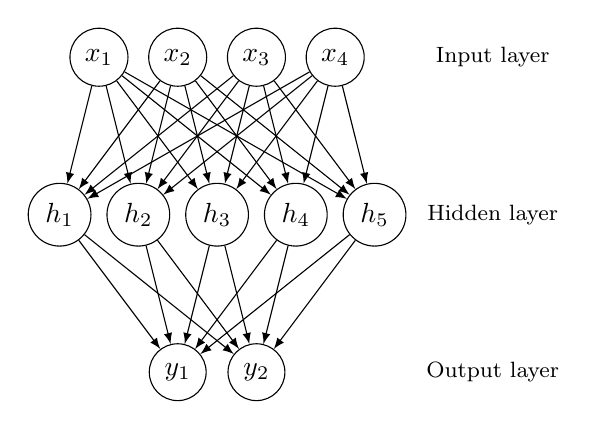
\begin{tikzpicture}
    \foreach \i in {1,2,3,4} {
      \node[circle,draw] at (\i,4) (x\i) {$x_{\i}$};
    }
    \foreach \i in {1,2,...,5} {
      \node[circle,draw] at ($(\i,2)-(0.5,0)$) (h\i) {$h_{\i}$};
      \foreach \j in {1,2,3,4} {
        \draw[-latex] (x\j) -- (h\i);
      }
    }
    \foreach \i in {1,2} {
      \node[circle,draw] at ($(\i,0)+(1,0)$) (y\i) {$y_{\i}$};
      \foreach \j in {1,2,...,5} {
        \draw[-latex] (h\j) -- (y\i);
      }
    }
    
    \node at (6,4) {\footnotesize Input layer};
    \node at (6,2) {\footnotesize Hidden layer};
    \node at (6,0) {\footnotesize Output layer};
\end{tikzpicture}

    \caption{Its traditional representation as a neural network}
    \label{fig:neuralnet}
  \end{subfigure}
\end{figure}

\bibliographystyle{chicago}
\bibliography{references}

\end{document}

